\section{Quantum Topics Justification}

%%%%%%%%%%%%%%%%%%%%%%%%%%%%%%%%%%%%%%%%%%%%%%%%%%%%%%%%%%%%%%%%%%%%%%%%%%%%%%%%%%%%%%%%%%%%%%%%%%%%%%%%%%%%%%%%%%%%%%%%
%%%%%%%%%%%%%%%%%%%%%%%%%%%%%%%%%%%%%%%%%%%%%%%%%%%%%%%%%%%%%%%%%%%%%%%%%%%%%%%%%%%%%%%%%%%%%%%%%%%%%%%%%%%%%%%%%%%%%%%%
\subsection{Motivation \& Teaching Strategy}

As meaningful introductory course into quantum computation, we must maximise the leverage of 
 classical competencies and existing curriculum components whilst respecting the varied backgrounds of our students.  
Cloud based quantum facilities now make practical skills attainable, 
however the field is still dominated by algebraic notations and intricate physical calculus. 
To engage a wider community of engineers and mathematicians,
we need to present only the core concepts and mathematical tools required to implement quantum algorithms.

\emph{cite Abhijith to make the point of this mindset and available material}

Through a cryptographic lens we see how analogue quantum phenomenon underpin key-distribution protocols,
and how the most celebrated realisation of digital quantum computing, in Shor's algorithm, 
breaks the one-way functions of asymmetric cryptography.
The temptation often leads straight to post-quantum encryption schemes, 
but we must first understand the quantum side clearly.  

%Why turn-away from cryptographic research areas and look at quantum algorithms more generally?
%The area of understanding new quantum algorithms, and reverse engineering classical algorithms \emph{cite{something}} is burgeoning.
%And the understanding if these new 

%Take, as an example, the \href{https://csrc.nist.gov/CSRC/media/Presentations/crystals-dilithium-round-3-presentation/images-media/session-1-crystals-dilithium-lyubashevsky.pdf}{CRYSTAL-Dilithium NIST "Schnorr-like” lattice-based signature scheme}.
%Schnorr's identification protocol \emph{cite{Schnorr:1990}} 
%\href{https://cybersecurity.springeropen.com/articles/10.1186/s42400-023-00198-1}{is an example a zero-knowledge protocol} 
%that need to convince a verifier knows the discrete logarithm \emph{I may have misunderstood the last point}.
%The hardness assumptions are based on the computational problems of the \emph{Shortest Vector Problem (SVP)} 
%and \emph{Closest Vector Problem (CVP)}.  
%We have jumped from the understanding of quantum phenomenon and promise and pitfalls of quantum technologies to
%a specialised topic in mathematics \emph{what's the best description of the topics around SPV and ZK}.  
%These are interesting a challenging topics, but should be introduced in their own way.

%But moving forward, with the introductory course, into more general quantum algorithms that are not directly applicable to cryptography
%provided it's own benefits.
%Firstly is, the current generation of analogue quantum annealing computers \emph{cite or reference D-Wave} are being used to attempt
%to break certain \emph{Substitution-Permutation Network (SNP)} problems.
%This demonstrates that a working understanding of quantum annealing and QUBO solvers is something that is at least in our bailiwick.
%More simply, we don't know how the next generation of quantum algorithms could be used to attack encryption protocols, 
%so rounding out the programme by looking more generally at these algorithms is justified. 


%%%%%%%%%%%%%%%%%%%%%%%%%%%%%%%%%%%%%%%%%%%%%%%%%%%%%%%%%%%%%%%%%%%%%%%%%%%%%%%%%%%%%%%%%%%%%%%%%%%%%%%%%%%%%%%%%%%%%%%%
%%%%%%%%%%%%%%%%%%%%%%%%%%%%%%%%%%%%%%%%%%%%%%%%%%%%%%%%%%%%%%%%%%%%%%%%%%%%%%%%%%%%%%%%%%%%%%%%%%%%%%%%%%%%%%%%%%%%%%%%
\subsection{Leveraging Classical Competencies}

%\emph{With the varied backgrounds of students we can't assume a core set of mental models, 
%	so don't skip the intro details, but move fast to get everyone up to speed.}

%\emph{This can be aided by leveraging core competencies within the existing curriculum; 
%	presenting a lot of algorithms will have analogies within disciplines already being presented.}

Because students enter with different backgrounds, we cannot assume shared mental models; 
we therefore start from fundamentals but move quickly.
Many quantum algorithms have direct analogues in topics already taught across the programme:

\begin{itemize}
	\item Quantum Machine learning techniques $\leftarrow$ linear‑algebra / kernel methods
	\item Post-quantum cryptography $\leftarrow$ number theory, lattice maths
	\item Quantum key distribution $\leftarrow$ information‑theory concepts
\end{itemize}

The aim of this section is to look at a practical quantum topic that a new student may be motivate to investigate;
for example quantum kernels in \emph{One-Class Support Vector Machines} (OC-SVMs) used for anomaly detection.
From deconstructing it, we look to reveal precisely what a student must master.
But some mathematics of quantum computation are non‑negotiable 
and we should visit some technical topics first with-out being pedagogic.

%\subsubsection{Leveraging Classical Competencies}

The topic was contrived to demonstrate several points,
one being that delivery of the quantum syllabus should draw on other competencies
that the student and programme curriculum provide.

The student should feel capable of being able to apply the core quantum principals to novel situations.  
The example here is of using a concepts of time and space complexities to estimate quantum computing resources.

%%%%%%%%%%%%%%%%%%%%%%%%%%%%%%%%%%%%%%%%%%%%%%%%%%%%%%%%%%%%%%%%%%%%%%%%%%%%%%%%%%%%%%%%%%%%%%%%%%%%%%%%%%%%%%%%%%%%%%%%
%%%%%%%%%%%%%%%%%%%%%%%%%%%%%%%%%%%%%%%%%%%%%%%%%%%%%%%%%%%%%%%%%%%%%%%%%%%%%%%%%%%%%%%%%%%%%%%%%%%%%%%%%%%%%%%%%%%%%%%%
\subsection{Foundational Topics}

Getting a solid grip on the mathematical underpinnings of quantum computation is key, 
and there is a balance between gaining mastery of these necessary skills and casting our net too widely.

%There are examples of introductions to quantum computations that eschew the starting with quantum concepts, 
%Lipton \cite{Lipton:2021}, Abhijith \cite{Abhijith:2022}, Ekert \href{https://arxiv.org/pdf/quant-ph/0011013}{Basic concepts in quantum computation}.
%Nielsen, on the other hand, introduce the concepts of quantum behaviour, the mathematical constructs needed to model these,
%and an application of entanglement in super-dense coding that is a good model to covering ground quickly \cite{Nielsen:2010}

%%%%%%%%%%%%%%%%%%%%%%%%%%%%%%%%%%%%%%%%%%%%%%%%%%%%%%%%%%%%%%%%%%%%%%%%%%%%%%%%%%%%%%%%%%%%%%%%%%%%%%%%%%%%%%%%%%%%%%%%
\subsubsection{Qubits \& State Spaces}

Starting with some mental models of quantum information and how it is distinct from classical information
and refreshing some linear algebra, matrix manipulation and polar notations will be needed.  
%We don't need to go into in-depth in descriptions of the main quantum particles, but 

We begin with physical examples of physical two‑level quantum systems, 
where out quantum particles have wtwo distinct states, such as a photon's horizontal or vertical polarization of its electromagnetic field, 
the electrons up or down spin state, and the trapped ion's high or low energy state.
And we can imagine we have some physical quantum machinery that is able to control the state of these particles.
This mental model gives a base for the core abstraction of quantum information and computation.

\begin{figure}[ht]
	\begin{adjustbox}{center}
		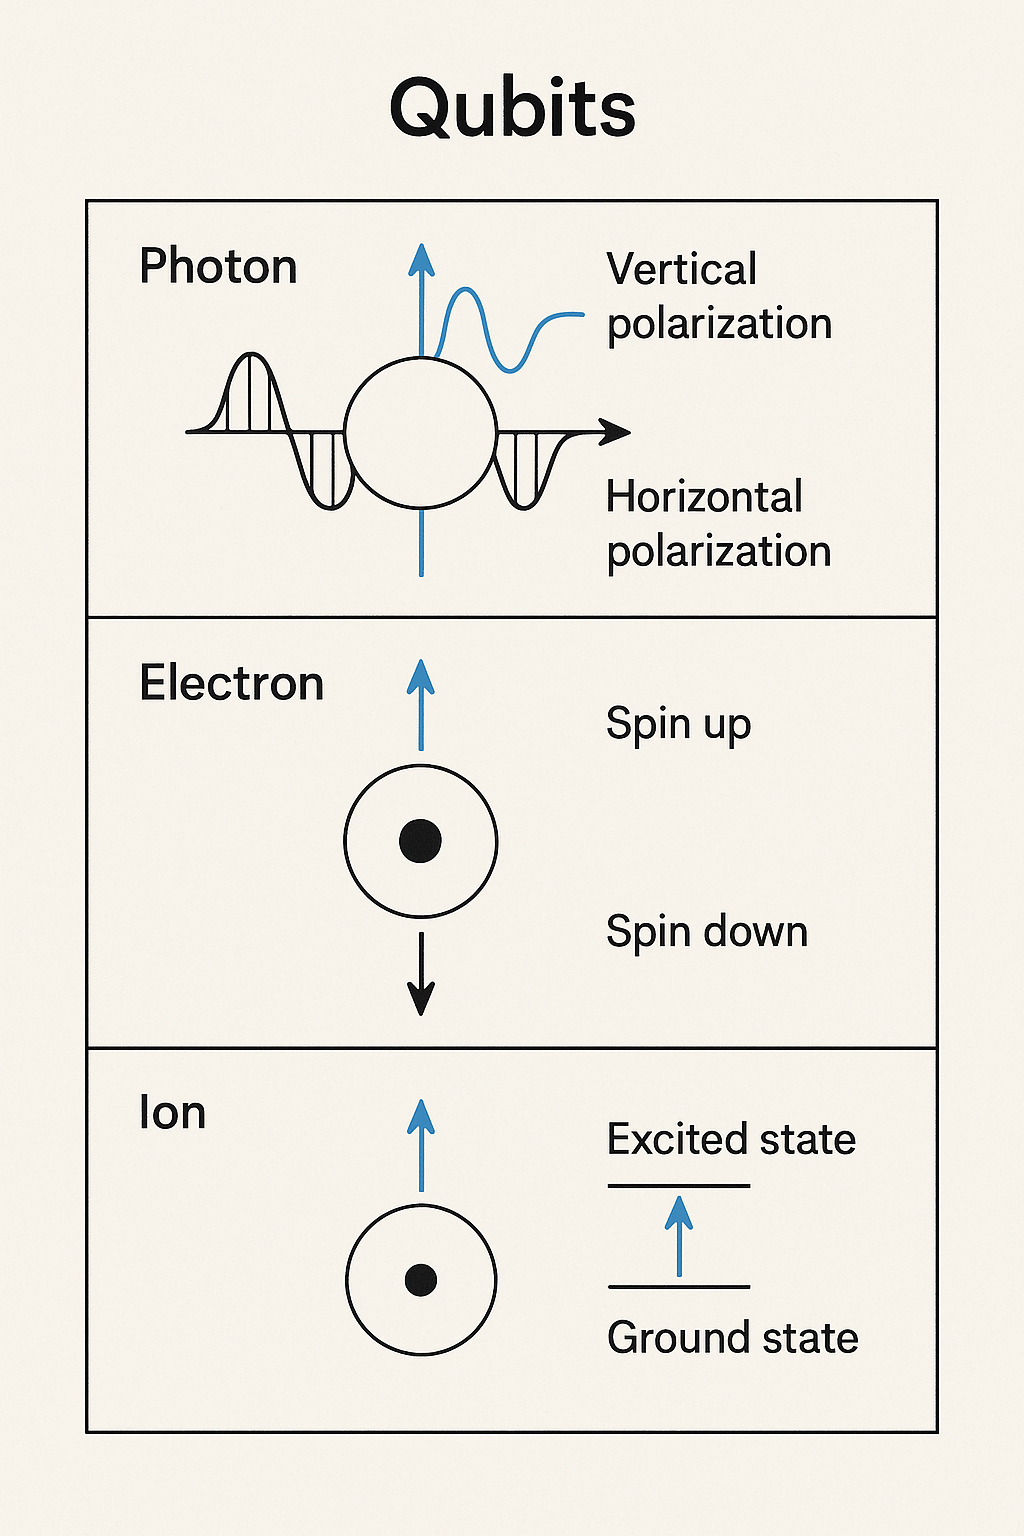
\includegraphics[width=0.3\textwidth, inner]{figures/physical_qubits_2.png}
	\end{adjustbox}
	\caption{Representation of physical qubit states} %\href{https://commons.wikimedia.org/wiki/File:Tolmukapea.jpg}{https://commons.wiki-\\media.org/wiki/File:Tolmukapea.jpg}.}
\label{fig:phys_qubit}
\end{figure}

These simple two level quantum systems have two states that we can label $\lvert0\rangle$ and $\lvert1\rangle$;
"horizontal" or "vertical", "up" or "down", "ground" or "excited".
We can then draw an analogy between a digital bit in a classical computer that has the states $0$ or $1$.
What is different about the information being manipulated in these two systems?
In a digital system we have a switch that we can flip from one state to another.
In quantum systems have something like a hi-fi balance knob that we can have either state,
or a mixed combination of the two.

In this framing, we have an amplitude, $\alpha$ and $\beta$, for each state, 
and the combined particle state is the vector $\lvert\psi\rangle = \alpha \lvert0\rangle + \beta \lvert1\rangle$.
Our system two level quantum system is a \emph{qubit} and it can be in a \emph{superposition} of the two states.

Graphically we can represent the combined state of these two special orthogonal \emph{computational basis states} 
as a point on a unit circle in a regular Euclidean space, which is a generalisation of a \emph{Hilbert space}.  

\begin{figure}[ht] 
	\begin{adjustbox}{center}
		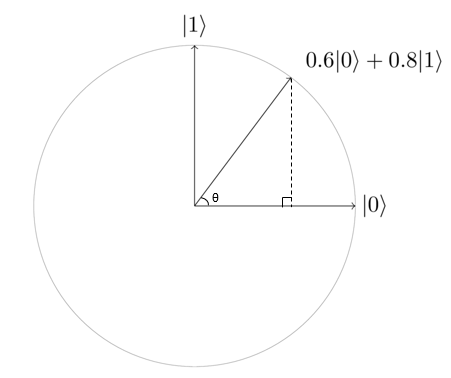
\includegraphics[width=0.3\textwidth, inner]{figures/unit-vector-2-d-hilbert-state.png}
	\end{adjustbox}
	\caption{$\lvert\psi\rangle$ as superposition of $\lvert0\rangle$ and $\lvert1\rangle>$ }
	\label{fig:2d_hilbert_space}
\end{figure}

We can in many cases think of $\alpha$ and $\beta$ as real numbers, but for they complex numbers, 
so this qubit space is described mathematically as a two-dimensional complex 
Hilbert space $\mathcal{H} : \mathbb{C}^2$ \cite{Preskill:2023} \cite{Nielsen:2010}.


%%%%%%%%%%%%%%%%%%%%%%%%%%%%%%%%%%%%%%%%%%%%%%%%%%%%%%%%%%%%%%%%%%%%%%%%%%%%%%%%%%%%%%%%%%%%%%%%%%%%%%%%%%%%%%%%%%%%%%%%
\subsubsection{Measurement \& Probability (Born rule)}

Limited Information from Measurement: A single measurement of an $n$-qubit state yields only $n$ bits of classical data, 
revealing only a \enquote{meager shadow} of the underlying quantum state \cite{Preskill:2023}.


Once we disturb this state $\lvert\phi\rangle$ by measuring our quantum particle, 
we will either see it in one of these basis states, states that we can measure and observe; 
horizontal or vertical polarization, up or down spin state, high or low energy levels.  

Whilst the system is isolated and unobserved, we can apply transforms, or computations, to the system,
and our qubit can evolve as a point on a sphere of possibilities, until we measure it's state as one of the two basis states;
a photon yielding "horizontal" or "vertical" polarisation.  
The final measurement outcome is inherently probabilistic; 
the probability of measuring $\lvert0\rangle$ is $\lvert\alpha\lvert^2|$, or $\lvert1\rangle$ $\lvert\beta\lvert^2|$.
So these co-ordinates $\alpha$ and $\beta$ have to obey certain rules, 
such as $\lvert\alpha\lvert^2 + \lvert\beta\lvert^2 = 1$; 
the final measurement of our photon guaranteed to be either "horizontal" or "vertical".

Because the $\lvert\alpha\lvert^2 + \lvert\beta\lvert^2 = 1$, we can effectively write our qubit state as \cite{Nielsen:2010}
$$\lvert\psi\rangle = cos \frac{\theta}{2} \lvert0\rangle + e^{i\varphi} sin \lvert1\rangle $$

The numbers $\theta$ and $\varphi$ define a point on a three dimensional \emph{Bloch sphere} 
that is useful initially for visualising a qubit state.

\begin{figure}[ht] 
	\begin{adjustbox}{center}
		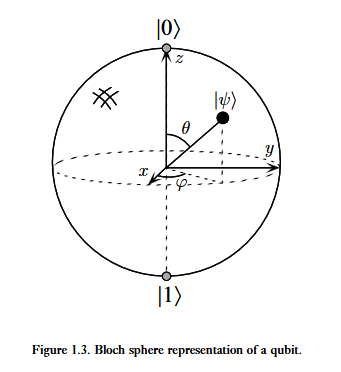
\includegraphics[width=0.3\textwidth, inner]{figures/blochsphere-nielsen-and-chuang-toc-and-chapter1-nov00.png}
	\end{adjustbox}
	\caption{Bloch sphere representation of a qubit }
	\label{fig:bloch_sphere}
\end{figure}

At later stages these can be developed into an understanding the benefits and difficulties each 
realisation of a quantum system.

%%%%%%%%%%%%%%%%%%%%%%%%%%%%%%%%%%%%%%%%%%%%%%%%%%%%%%%%%%%%%%%%%%%%%%%%%%%%%%%%%%%%%%%%%%%%%%%%%%%%%%%%%%%%%%%%%%%%%%%%
\subsubsection{Unitary Dynamics \& Gate Model}

If we know that the two vectors encoding these two basis states of our vector space are
$$\lvert0\rangle = \begin{bmatrix} 1 \\ 0 \end{bmatrix} \quad \textrm{and} \quad \lvert1\rangle = \begin{bmatrix} 0 \\ 1 \end{bmatrix}$$

then for the mathematically inclined giving the qubit state representation as:

$$\lvert\phi\rangle = \begin{bmatrix} \alpha \\ \beta \end{bmatrix} = \alpha\lvert0\rangle + \beta\lvert1\rangle$$
could be enlightening.

One postulate of quantum mechanics states that the evolution of an isolated system is unitary:
$$ \lvert \psi'\rangle = U \lvert \psi \rangle, \quad U^{\dagger} U = I$$

represents the notion that applying an operator twice leaves us in the initial state.

Unitary gates are therefore \textbf{reversible}, unlike many classical logic gates. [Consider moving Toffoli example here for continuity.]


We will define more exactly what a quantum circuit is, 
but at this point we can understand it from the our general knowledge of classical digital circuits,
transforming electronic states, doing our bidding in the computers that surround us in our daily lives.
Except that we are using quantum machinery to transform quantum states.

One of the postulates of quantum dynamics is that the evolution of a closed quantum system is described by a
\emph{unitary transformation} \cite{Nielsen:2000}.  
Given a state of a system at $t_1$ as $|\psi\rangle$, it is related to the state $|\psi'\rangle$ at time $t_2$ 
by a unitary operator:

$$|\psi'\rangle = U|\psi\rangle$$

Unitary transforms are invertible by their \emph{conjugate transpose} $U^\dag$.  
Applying the conjugate transpose, we end up where we started, 
which is the same as applying the identity matrix $I$ to our state, leaving the state unchanged:

$$UU^\dag = I$$

The practical upshot is that all transforms applied to our quantum state $|\psi\rangle$ has to be a unitary transform.
And that every tiny step in an evolving quantum system can be run backwards exactly.

Because of the rules of unitary transformations, at this point, we can imagine our quantum algorithm, or circuit, 
as one large unitary transformation, taking our initial quantum state into our desired final state.


%%%%%%%%%%%%%%%%%%%%%%%%%%%%%%%%%%%%%%%%%%%%%%%%%%%%%%%%%%%%%%%%%%%%%%%%%%%%%%%%%%%%%%%%%%%%%%%%%%%%%%%%%%%%%%%%%%%%%%%%
\subsubsection{Entanglement \& Tensor Products}

Not all, arbitrary, transformations are valid (irreversible ones especially, and we will touch on that later).
and an application of entanglement in super-dense coding that is a good model to covering ground quickly \cite{Nielsen:2010}

%\href{https://www.forbes.com/sites/chadorzel/2017/02/28/how-do-you-create-quantum-entanglement/}{how-do-you-create-quantum-entanglement}

\emph{Quantum Registers}

In quantum computing a \emph{quantum register} is a system of  \cite{Lipton:2021} (p140).


%%%%%%%%%%%%%%%%%%%%%%%%%%%%%%%%%%%%%%%%%%%%%%%%%%%%%%%%%%%%%%%%%%%%%%%%%%%%%%%%%%%%%%%%%%%%%%%%%%%%%%%%%%%%%%%%%%%%%%%%
\subsubsection{Noise, Decoherence \& Error Correction}

%\emph{Estimating Gates and Circuit Depth}

%\emph{Note: the paper used QISKIT quantum simulator.  The paper has the shot count, but can we see the noise applied?}

%describe shot count; shot noise and statistical error-kernel variance shows up directly in OC-SVM decision boundaries.


%\subsubsection{Primitives to Support Quantum Kernel Computations}

%Now we look at the quantum kernel computation itself.  
%We are not going to analyse the 

%which often involves measurement techniques like the SWAP test, implied by overlap/fidelity calculations


%%%%%%%%%%%%%%%%%%%%%%%%%%%%%%%%%%%%%%%%%%%%%%%%%%%%%%%%%%%%%%%%%%%%%%%%%%%%%%%%%%%%%%%%%%%%%%%%%%%%%%%%%%%%%%%%%%%%%%%%
\subsection{Core Algorithmic Primitives}

The ubiquity of Shor's algorithm for integer factorisation and finding discrete logarithms,
interestingly means that we need a wide range of supporting methods early.  
This paper demonstrates several major building blocks that are reused across subsequent algorithms.

Shor implements an existing, classical, Sch\"{o}nhage-Strassen fast multiplication algorithm.
This uses a Fourier transform, to find order of a function.  
When factoring $M = pq$, $p$ and $q$ being distinct prime numbers,
we can define a function $f_x(a) = (x^a mod M)$, which because of the modular arithmetic, is periodic.
That is, given $r' = (p-1)(q-1)$, $x^{a+r'} mod M) = x^a mod M$ because, as p and q are prime, 
from the Chinese Remainder Theorem, $x^{p-1} \equiv 1 mod p$ and  $x^{q-1} \equiv 1 mod q$.
So the function has a minimal period $r$ that divides $r'$.  
To find the smallest integer $r$ such that $x^r = 1 mod M$, 
we show that $f_x(0),..., f_x(r-1)$ are distinct.  
At this point we just need to note that after implementing the modular exponentiation,
Shor uses a $Quantum Fourier Transform$ (QFT) to find the period of the function \cite{Shor:1996}. 

%%%%%%%%%%%%%%%%%%%%%%%%%%%%%%%%%%%%%%%%%%%%%%%%%%%%%%%%%%%%%%%%%%%%%%%%%%%%%%%%%%%%%%%%%%%%%%%%%%%%%%%%%%%%%%%%%%%%%%%%
\subsubsection{State Preparation \& QRAM Issues}

Shor's algorithm demonstrates the main quantum computation stages \cite{Nielsen:2010}:

Encoding classical data into quantum states efficiently can be non-trivial, 
sometimes requiring circuits whose complexity scales with the classical data size, despite the memory compression in qubits

\subsubsection{Fourier / Phase Estimation}

With integer factorization, it is easy to verity is necessary to boost the probability of success \cite{Lipton:2021}.
Shor's algorithm succeeds with a probability of less than one.


%%%%%%%%%%%%%%%%%%%%%%%%%%%%%%%%%%%%%%%%%%%%%%%%%%%%%%%%%%%%%%%%%%%%%%%%%%%%%%%%%%%%%%%%%%%%%%%%%%%%%%%%%%%%%%%%%%%%%%%%
\subsubsection{Amplitude Amplification}

Like many quantum algorithms, this 
\emph{Amplitude Amplification} (AA) \cite{Dalzell:2023} is the probabilistic technique of 
repeating the call and to a unitary that verifies success of the call, to boost the success probability
closer to 1.

%We have already made the point that quantum computing applies reversible unitary transformations to the quantum state.  
%The modular exponentiation arithmetic is a 

%The technique uses 
%The reversible modular exponentiation 

%So the exponential improvement of  over the classical version is 


%We can view the modular \cite{Dalzell:2023}

%%%%%%%%%%%%%%%%%%%%%%%%%%%%%%%%%%%%%%%%%%%%%%%%%%%%%%%%%%%%%%%%%%%%%%%%%%%%%%%%%%%%%%%%%%%%%%%%%%%%%%%%%%%%%%%%%%%%%%%%
\subsubsection{Block Encoding \& QSVT}

This is in contrast to Block-encoding, 
helps define certain ideas that are needed to engage with quantum computing as $C = U_1 .. U_n$. 
The core insight being that classical computing can be realised by quantum machinery, 
not by making the classical computational reversible (boolean functions can be made reversible\cite{Bennett:1989}),
but by admitting that the dynamics of a subsystem with a quantum system can be non-unitary.

%%%%%%%%%%%%%%%%%%%%%%%%%%%%%%%%%%%%%%%%%%%%%%%%%%%%%%%%%%%%%%%%%%%%%%%%%%%%%%%%%%%%%%%%%%%%%%%%%%%%%%%%%%%%%%%%%%%%%%%%
%%%%%%%%%%%%%%%%%%%%%%%%%%%%%%%%%%%%%%%%%%%%%%%%%%%%%%%%%%%%%%%%%%%%%%%%%%%%%%%%%%%%%%%%%%%%%%%%%%%%%%%%%%%%%%%%%%%%%%%%
\subsection{Case‑Study Back‑Mapping}

In a recent paper, \citetitle{Poutre:2024}, \citeauthor{Poutre:2024} \cite{Poutre:2024} use a modified 
\emph{Large Language Model} (LLM) \emph{Transformer} auto-encoder architecture to 
\enquote{learn rich temporal limit order book subsequence representations}.  
From this trained encoder network they then train an OC-SVM to detect financial fraud, with seemingly good results.

A Support Vector Machine (SVM) is a machine learning algorithm used for classification and regression tasks.  
It is widely used in text classification and image recognition, for example.
Typically they are used in a supervised learning context where labelled data is available to fit the model.

The primary aim of the SVM is to separate data points into distinct classes by finding the best boundary that divides them.
In a 2-D space this boundary is a line, in 3-D a plane, and in higher dimensional spaces, a \emph{hyperplane}.
This boundary is found by maximising the distance between the boundary and the nearest data points in each class;
these '\emph{support vectors}' define the hyperplane. 
If the data isn't neatly separable, 
the SVM uses an mathematical transform to project the data into a higher dimensional space, 
where a clear boundary can be found.
These transformations are called \emph{kernels}, and there are many classes of kernels available.

\citeauthor{Scholkopf:1999} in 1999 \cite{Scholkopf:1999} introduced OC-SVMs as a variant of SVMs designed for one task;
outlier or novelty detection.
By focusing on distinguishing between 'normal' data and everything else, 
and only forming a hyperplane using a single class of data during training, 
they can used for semi or un-supervised applications.

\citeauthor{Kyriienko:2022} \cite{Kyriienko:2022} in 2022 developed an application of OC-SVMs using quantum kernels.
In their paper they successfully used a simulator of 20 qubits (one qubit per dataset feature)
on a reduced data set, and most interestingly, performed analysis on the training and inference times needed, 
and in the process demonstrating that the quadratic scaling of the Gram matrix evaluation 
made their approach infeasible on the full dataset.

Promising work has been done to reduce the time-complexity of the evaluation of the Gram matrix, 
by \citeauthor{Kolle:2023} \cite{Kolle:2023}, using randomised measurements and variable subsampling.

The aim of the studedent's paper would be to investigate whether quantum kernel OC-SVM algorithms are practical 
given our reliance of NISQ machinery.
It is well known that these devices have the constraints of having only limited number of qubit to represent model state,
and that they introduce errors that constrain the complexity and depth of circuits that they can run \cite{Preskill:2018}.
In their paper, P\"{o}utre state that their autoencoder of had a dimensionality of 128 \cite{Poutre:2024},
far larger that the feature set of 20 used by Kyriienko \cite{Kyriienko:2022}.
With the recent announcement by Google that their new 105 qubit \emph{Willow} processor has
achieved below threshold quantum error correction \cite{Google:Willow:2024}, the main body of this report is to: 
(1) reanalyse the training and inference times by Kyriienko assuming the performance stated in Google's research;
(2) assess whether the new hardware could be used to apply the OC-SVM algorithm to the P\"{o}utre paper dataset
and to estimate for the training and inference times.


Many sources emphasise the importance of "end-to-end" analysis when evaluating quantum \cite{Dalzell:2023} \cite{Morales:2025}
algorithms, including classical and quantum overheads (state preparation, measurement, error mitigation),
to assess the feasibility and potential quantum advantage of these solutions.  
Resource estimation (qubits, gates, runtimes, measurement shots) 
is a key aspect of understanding challenges and limitations,
and hence a desirable outcome for new practitioners.

%%%%%%%%%%%%%%%%%%%%%%%%%%%%%%%%%%%%%%%%%%%%%%%%%%%%%%%%%%%%%%%%%%%%%%%%%%%%%%%%%%%%%%%%%%%%%%%%%%%%%%%%%%%%%%%%%%%%%%%%
\subsubsection{Hybrid Processing Pipelines}

A second point is that details from the paper by \citeauthor{Kyriienko:2022} 
bring up an interesting point that may not be obvious from the abstract. 
Their technique is to apply only the kernel transform using quantum techniques, 
not to generate, or embed, the Gram matrix in a quantum vector state.
The constructing the Gram matrix, as well as the autoencoder, use classic computing systems. 
And as in Shor's original quantum paper on discrete logarithms and factoring \cite{Shor:1996},
this is an example of a hybrid classical-quantum computing system \cite{Preskill:2023}.

There are commercial realities \emph{(and skills shortages anecdotally from workshop I went to)}
that can have direct tie-ins to data engineering skills being developed with the full curriculum.

In this hybrid model, 
the quantum system acts as a co-processor, executing specific sub-routines that are expected to offer quantum advantage.
The classical computer orchestrates data preparation, algorithm set-up, and post-processing tasks.
There are parallels to the engineering challenges of \emph{Extract, Transform, Load} (ETL) 
in classical machine learning data pipelines and GPU workflows.

%%%%%%%%%%%%%%%%%%%%%%%%%%%%%%%%%%%%%%%%%%%%%%%%%%%%%%%%%%%%%%%%%%%%%%%%%%%%%%%%%%%%%%%%%%%%%%%%%%%%%%%%%%%%%%%%%%%%%%%%
\subsubsection{Exposure to Commercial Platforms}

\emph{Commercial offerings are available, so there are options to fold practical experience into the course options.
	Hybrid processing pipelines examples; would need to introduce products (move to a later part of this section on SDKs)}

\begin{itemize}
	\item \href{https://docs.aws.amazon.com/braket/latest/developerguide/braket-what-is-hybrid-job.html}
	{AWS Braket Hybrid jobs}
	\item \href{https://pennylane.ai/qml/demos/tutorial_quantum_transfer_learning}
	{Pennylane hybrid Quantum Transfer Learning example}
	\item \href{https://ml2quantum.com/2020/05/22/zapata-orquestra/}
	{Zapata Orquestra; I haven't looked into yet}
	\item \href{https://docs.quantum.ibm.com/api/qiskit-ibm-runtime/0.16/runtime-service
	}{IBM Qiskit Runtime allows an aspect or orchestration}
\end{itemize}

%%%%%%%%%%%%%%%%%%%%%%%%%%%%%%%%%%%%%%%%%%%%%%%%%%%%%%%%%%%%%%%%%%%%%%%%%%%%%%%%%%%%%%%%%%%%%%%%%%%%%%%%%%%%%%%%%%%%%%%%
\subsubsection{Block Encoding and Quantum Linear System Solvers}

When we were talking about quantum computation first downside of this imposed rule, is that not all, arbitrary, transformations are valid 
(irreversible ones especially, and we will touch on that later).

The pressing problem for machine learning, Gram matrices for SVM kernels, 
Hamiltonian matrices describing a desired evolution, and general data vectors, are generally non-unitary.
If we want to run our Netflix recommender system in our brave new, fully quantum (none of this hybrid rubbish), world,
how do we keep the physics happy, whilst computing the matrix we actually want?

Without going into the details, but typically by introducing additional quantum registers, or \emph{ancillas}, 
there is a more advanced technique called \emph{Block Encoding} (BE) that can embed a, possibly non-unitary, matrix $A$ 
into a larger unitary $U$ \cite{Low:2017}.

$$
U = \begin{bmatrix} A & \ast \\ \ast & \ast \end{bmatrix}
$$

\emph{There is probably not much use here to introduce other precursor 
algorithms, such as the original \emph{Quantum Linear System Solver} (QLSS) by \citeauthor{Harrow:2009} \cite{Harrow:2009},
or to look at the history of block encoding from Berry, Childs, Cleve, Kothari and others, 
showing that you can simulate sparse Hamiltonians by writing them as linear combinations of short unitaries,
or looking at other more wide spread applications \emph{cite 2018 Gilyen, Su, Low \& Wiebe} 
via Quantum Singular Value Transformation (QSVT) 
where they apply lblock encoding with signal processing techniques, developing a single unifying technique} 
